\part{Python Management}

% LaTeX Canvas: Chapter Outline
\chapter{Package Management}
\label{ch:pkg-mgmt}

\section*{Purpose}
Package management is the discipline of installing and updating third-party software (libraries) in a way that is consistent, reproducible, and unlikely to break your work. For novices, the most common failure mode is mixing global installs, different Python interpreters, and ad-hoc updates until nothing imports. This chapter teaches a stable workflow using project-level environments, clear dependency records, and a conflict-resolution playbook.

\section*{Learning objectives}
By the end of this chapter, a reader should be able to:
\begin{enumerate}
\item Explain what a \textbf{package}, \textbf{dependency}, and \textbf{environment} are.
\item Choose between \texttt{conda} and \texttt{pip} for a given situation.
\item Create, activate, and remove isolated environments (conda environments and/or \texttt{venv}).
\item Install packages with good hygiene (no `random global installs'', avoid base/root env).
  \item Record dependencies for reproducibility (\texttt{environment.yml}, \texttt{requirements.txt}, optional lockfiles).
  \item Diagnose `it worked yesterday'' failures: wrong interpreter, wrong environment, conflicts.
\item Resolve dependency conflicts using solver output, pinning, and environment recreation.
\item Apply maintenance practices: updates, audits, and cleaning without breaking environments.
\end{enumerate}

\section*{Running theme: environments are disposable, projects are not}
Your project should be stable because it describes what it needs. If an environment breaks, you should be able to recreate it.

\section{Mental models and vocabulary}
\subsection{Packages and dependencies}
\begin{itemize}
\item \textbf{Package:} third-party code you install (e.g., \texttt{pandas}).
\item \textbf{Dependency:} another package your package needs.
\item \textbf{Version constraints:} rules like \texttt{>=}, \texttt{<}, \texttt{==} that restrict compatible versions.
\end{itemize}

\subsection{Environments and interpreters}
\begin{itemize}
\item A Python \textbf{interpreter} runs your code (and determines where packages are installed).
\item An \textbf{environment} is an isolated set of installed packages tied to a specific interpreter.
\item You can have many environments on one computer; each project should use one.
\end{itemize}

\subsection{Reproducibility artifacts}
\begin{itemize}
\item \texttt{environment.yml}: conda-style environment specification.
\item \texttt{requirements.txt}: pip-style install list.
\item \textbf{Lockfile:} a fully resolved, exact list of versions for repeatable installs.
\end{itemize}

\section{Choosing tools: \texttt{conda} vs \texttt{pip} vs \texttt{venv}}
\subsection{What conda is good at}
\begin{itemize}
\item Cross-language, compiled dependencies (e.g., scientific stacks, system libraries).
\item Environments that include non-Python packages.
\item Solving complex dependency graphs across compiled packages.
\end{itemize}

\subsection{What pip is good at}
\begin{itemize}
\item Installing Python packages from PyPI.
\item Lightweight environments using the standard library \texttt{venv}.
\item Working with Python packaging metadata (\texttt{pyproject.toml}, wheels).
\end{itemize}

\subsection{Practical student guidance}
\begin{itemize}
\item If your course provides a conda environment file, use conda.
\item If a library is only on PyPI, use pip (inside an environment).
\item Do not install packages globally for coursework.
\end{itemize}

\section{Baseline hygiene rules (non-negotiable)}
\subsection{Rule 1: never work in the base/root conda environment}
\begin{itemize}
\item Keep base/root for conda itself.
\item Create a separate environment per project.
\end{itemize}

\subsection{Rule 2: one project, one environment}
\begin{itemize}
\item Avoid ``one giant environment for everything''.
\item Name environments clearly (e.g., \texttt{ds101-week3}, \texttt{housing-audit}).
\end{itemize}

\subsection{Rule 3: prefer explicit specs over memory}
\begin{itemize}
\item Record dependencies in a file in the project repository.
\item Make install steps repeatable.
\end{itemize}

\subsection{Rule 4: avoid mixing managers casually}
\begin{itemize}
\item If you combine conda and pip: install as much as possible with conda first.
\item After using pip inside a conda environment, prefer recreating the environment rather than adding more conda packages.
\end{itemize}

\section{Core workflows with conda}
\subsection{Create and activate an environment}
\begin{verbatim}
conda create -n myproj python=3.12
conda activate myproj
\end{verbatim}

\subsection{Install, update, remove}
\begin{verbatim}
conda install pandas numpy
conda update pandas
conda remove pandas
\end{verbatim}

\subsection{Search and inspect}
\begin{itemize}
\item Search packages, inspect what is installed.
\item Confirm which environment is active before installing.
\end{itemize}

\subsection{Channels and channel priority (why you should care)}
\begin{itemize}
\item Channels are sources of packages; mixing channels can cause incompatibilities.
\item Prefer a consistent channel strategy for a project.
\item When using community channels (e.g., conda-forge), adopt strict channel priority to reduce incompatibilities.
\end{itemize}

\subsection{Exporting and sharing environments}
\begin{itemize}
\item Export an environment spec to share with teammates.
\item Store the spec (not the whole environment folder) in version control.
\end{itemize}

\subsection{Cleaning and cache hygiene (cautious)}
\begin{itemize}
\item Conda caches downloaded packages; cleaning can reclaim space.
\item Cleaning can have side effects; do it intentionally and only when needed.
\end{itemize}

\section{Core workflows with \texttt{venv} + \texttt{pip}}
\subsection{Create and activate a \texttt{venv}}
\begin{verbatim}
python -m venv .venv

# activate (platform-specific)

\end{verbatim}

\subsection{Install and record dependencies}
\begin{verbatim}
python -m pip install --upgrade pip
python -m pip install pandas
python -m pip freeze > requirements.txt
\end{verbatim}

\subsection{Recreate an environment from a requirements file}
\begin{verbatim}
python -m venv .venv

# activate

python -m pip install -r requirements.txt
\end{verbatim}

\subsection{Sanity checks}
\begin{itemize}
\item Confirm \texttt{which python} / \texttt{where python} points inside the environment.
\item Use \texttt{pip check} to detect inconsistent installs.
\end{itemize}

\section{Dependency conflicts: what they are and why they happen}
\subsection{The conflict pattern}
\begin{itemize}
\item You request package A and package B.
\item A requires version range of C; B requires a different version of C.
\item No single version satisfies both constraints.
\end{itemize}

\subsection{Symptoms novices see}
\begin{itemize}
\item Install fails with ``ResolutionImpossible'' (pip) or solver errors (conda).
\item Imports fail after an upgrade.
\item Runtime errors due to incompatible versions.
\end{itemize}

\section{Conflict-resolution playbook (a disciplined sequence)}
\subsection{Step 0: stop making it worse}
\begin{itemize}
\item Do not keep trying random installs.
\item Record the exact error output.
\end{itemize}

\subsection{Step 1: verify you are in the right environment}
\begin{itemize}
\item Confirm environment activation.
\item Confirm interpreter path and package locations.
\end{itemize}

\subsection{Step 2: reduce the problem}
\begin{itemize}
\item Try installing the smallest set of packages that triggers the conflict.
\item Install packages in one command when possible so the solver sees the full set.
\end{itemize}

\subsection{Step 3: read the solver's explanation}
\begin{itemize}
\item Identify the conflicting dependency (the shared package with incompatible constraints).
\item Identify which packages are forcing the constraints.
\end{itemize}

\subsection{Step 4: choose a strategy}
\begin{description}
\item[Pin a compatible version] Constrain one or more packages to versions known to work.
\item[Relax a constraint] If you pinned something unnecessarily, unpin it.
\item[Change channels/builds] In conda, ensure consistent channels and strict priority.
\item[Split environments] If two tools fundamentally conflict, they may need separate envs.
\item[Recreate the environment] Often fastest and cleanest once an environment is messy.
\end{description}

\subsection{Step 5: verify with a smoke test}
\begin{itemize}
\item Import key libraries.
\item Run a minimal script/notebook.
\item Re-run tests if available.
\end{itemize}

\section{Mixing conda and pip safely (when you must)}
\subsection{The recommended order}
\begin{enumerate}
\item Create a new conda environment.
\item Install as many dependencies as possible with conda.
\item Use pip for packages unavailable via conda.
\item If you later need more conda packages, consider recreating the environment.
\end{enumerate}

\subsection{Recording mixed dependencies}
\begin{itemize}
\item Keep conda dependencies in \texttt{environment.yml}.
\item Keep pip-only dependencies as a pip section or a separate \texttt{requirements.txt}.
\end{itemize}

\section{Reproducible environments: pins, constraints, and lockfiles}
\subsection{Pins vs ranges}
\begin{itemize}
\item Pins (\texttt{==}) maximize repeatability but can reduce upgradability.
\item Ranges (\texttt{>=,<}) allow updates but may introduce drift.
\item Teach a project policy: coursework often benefits from tighter pins.
\end{itemize}

\subsection{Constraints files (pip concept)}
\begin{itemize}
\item Separate `what to install'' from `allowed versions''.
\item Useful for controlling transitive dependencies.
\end{itemize}

\subsection{Lockfiles}
\begin{itemize}
\item Why: avoid solving at install time; install exactly known-good versions.
\item Conda: generate lockfiles for platforms.
\item Pip ecosystem: lockfile tools exist; understand the concept and when your course uses one.
\end{itemize}

\section{Package management hygiene over time}
\subsection{Updates (intentional, not accidental)}
\begin{itemize}
\item Update deliberately: ``why am I updating?''
\item Prefer updating in a fresh environment or on a branch.
\item After updates: run smoke tests.
\end{itemize}

\subsection{Auditing your environment}
\begin{itemize}
\item Check inconsistencies (pip).
\item Identify unused packages (conceptual).
\item Keep dependency lists minimal.
\end{itemize}

\subsection{Avoiding common foot-guns}
\begin{itemize}
\item Do not use \texttt{pip --user} for project work.
\item Do not run pip outside an active environment.
\item Avoid reinstalling random versions until imports succeed.
\item Avoid ``works on one machine'' by storing environment specs.
\end{itemize}

\section{Troubleshooting guide (novice-oriented)}
\subsection{``ModuleNotFoundError''}
\begin{itemize}
\item Installed into the wrong environment.
\item Wrong interpreter selected (IDE/kernel mismatch).
\item Fix: confirm interpreter path; reinstall in the active env.
\end{itemize}

\subsection{``It installed, but now something else broke''}
\begin{itemize}
\item A dependency was upgraded/downgraded.
\item Fix: inspect versions; consider reverting or recreating the environment.
\end{itemize}

\subsection{Conda solver is slow or failing}
\begin{itemize}
\item Too many channels or inconsistent channel priority.
\item Conflicting constraints.
\item Fix: use strict channel priority and simplify requirements.
\end{itemize}

\subsection{Pip is backtracking forever}
\begin{itemize}
\item Pip is searching for a compatible version set.
\item Fix: add constraints/pins, or start from a clean environment.
\end{itemize}

\section{Worked examples (outline)}
\subsection{Example 1: Create a clean conda environment for a project}
\begin{itemize}
\item Create env, install core packages.
\item Export environment spec.
\item Recreate from spec on a second machine.
\end{itemize}

\subsection{Example 2: Use pip inside a venv for a small script}
\begin{itemize}
\item Create \texttt{.venv}, install two packages.
\item Freeze to \texttt{requirements.txt}.
\item Recreate and verify with a smoke test.
\end{itemize}

\subsection{Example 3: Diagnose a dependency conflict}
\begin{itemize}
\item Trigger a conflict.
\item Read the error output to find the incompatible dependency.
\item Resolve by pinning or splitting environments.
\end{itemize}

\subsection{Example 4: Notebook/IDE kernel mismatch}
\begin{itemize}
\item Symptom: notebook cannot import a package that the terminal can.
\item Diagnosis: wrong kernel/interpreter.
\item Fix: select the correct kernel; verify versions.
\end{itemize}

\section{Templates}
\subsection{Template A: Minimal \texttt{environment.yml} (conceptual)}
\begin{verbatim}
name: myproj
channels:

* conda-forge
* defaults
  dependencies:
* python=3.12
* pandas
* numpy
* pip
* pip:

  * some-pypi-only-package
    \end{verbatim}

\subsection{Template B: Environment ``smoke test''}
\begin{verbatim}
python -c "import sys; print(sys.version)"
python -c "import pandas as pd; print(pd.**version**)"
python -m pip check
\end{verbatim}

\subsection{Template C: Project dependency policy (student-friendly)}
\begin{verbatim}

* Every project has an environment file.
* No installs in base/root.
* All installs happen through conda (preferred) or pip (only in an env).
* If the environment breaks, recreate it.
* Before submission, restart kernel/run all notebooks to confirm the env works.
  \end{verbatim}

\section{Exercises}
\begin{enumerate}
\item Create a new conda environment, install two packages, and export an environment spec.
\item Create a new \texttt{venv}, install one package, write \texttt{requirements.txt}, and recreate it.
\item Intentionally install conflicting requirements in a fresh env; read the error and identify the conflicting dependency.
\item Fix the conflict by pinning one package version or splitting into two envs.
\item Demonstrate a kernel/interpreter mismatch and then correct it.
\item Write a one-page ``environment README'': how to create, activate, and verify the environment.
\end{enumerate}

\section{One-page checklist}
\begin{itemize}
\item I do not install packages globally for projects.
\item I can create and activate a project environment.
\item I can confirm which \texttt{python} and \texttt{pip} I am using.
\item I record dependencies in a file tracked with the project.
\item I understand how conflicts arise and can read solver output.
\item I can resolve conflicts by pinning, simplifying, or recreating an environment.
\item I use conda channels deliberately and prefer strict priority when appropriate.
\item I verify environments with a small smoke test before important work.
\end{itemize}

\appendix
\section{Quick reference: commands students use most}
\subsection{conda}
\begin{verbatim}
conda create -n NAME python=3.12
conda activate NAME
conda install PKG
conda update PKG
conda env export > environment.yml
conda env remove -n NAME
\end{verbatim}

\subsection{pip (inside an env)}
\begin{verbatim}
python -m pip install PKG
python -m pip install -r requirements.txt
python -m pip freeze > requirements.txt
python -m pip check
\end{verbatim}

The steps for downloading, installing, using, and maintaining Python with \conda will differ based on your operating system. \conda can be used by Macs running macOS (OS X), PCs running Windows, and PCs running Linux. \conda cannot be installed or used on managed operating systems like ChromeOS (\textit{e.g.}, Chromebooks) or iOS (\textit{e.g.}, iPads). It is unlikely that you will be able to install or configure \conda yourself on ``managed'' computers like those found in libraries or computer labs.

\conda is only a package manager: it does not include Python or any of its libraries for data retrieval, analysis, visualization, \textit{etc}. At this stage you can either (1) install Anaconda Individual Edition\footnote{\url{https://www.anaconda.com/products/individual}} that includes hundreds of popular libraries and their dependencies or (2) install ``miniconda''\footnote{\url{https://docs.conda.io/en/latest/miniconda.html}} and choose which libraries you want installed. In either case, \conda will be the package manager that helps you install and maintain these libraries. Figure~\ref{fig:conda_mini_ana} captures the relationships between \conda, miniconda, and Anaconda. Anaconda is easier to install and harder to keep up-to-date while miniconda is harder to install and a easier to keep up-to-date.

\begin{marginfigure}
    \centering
    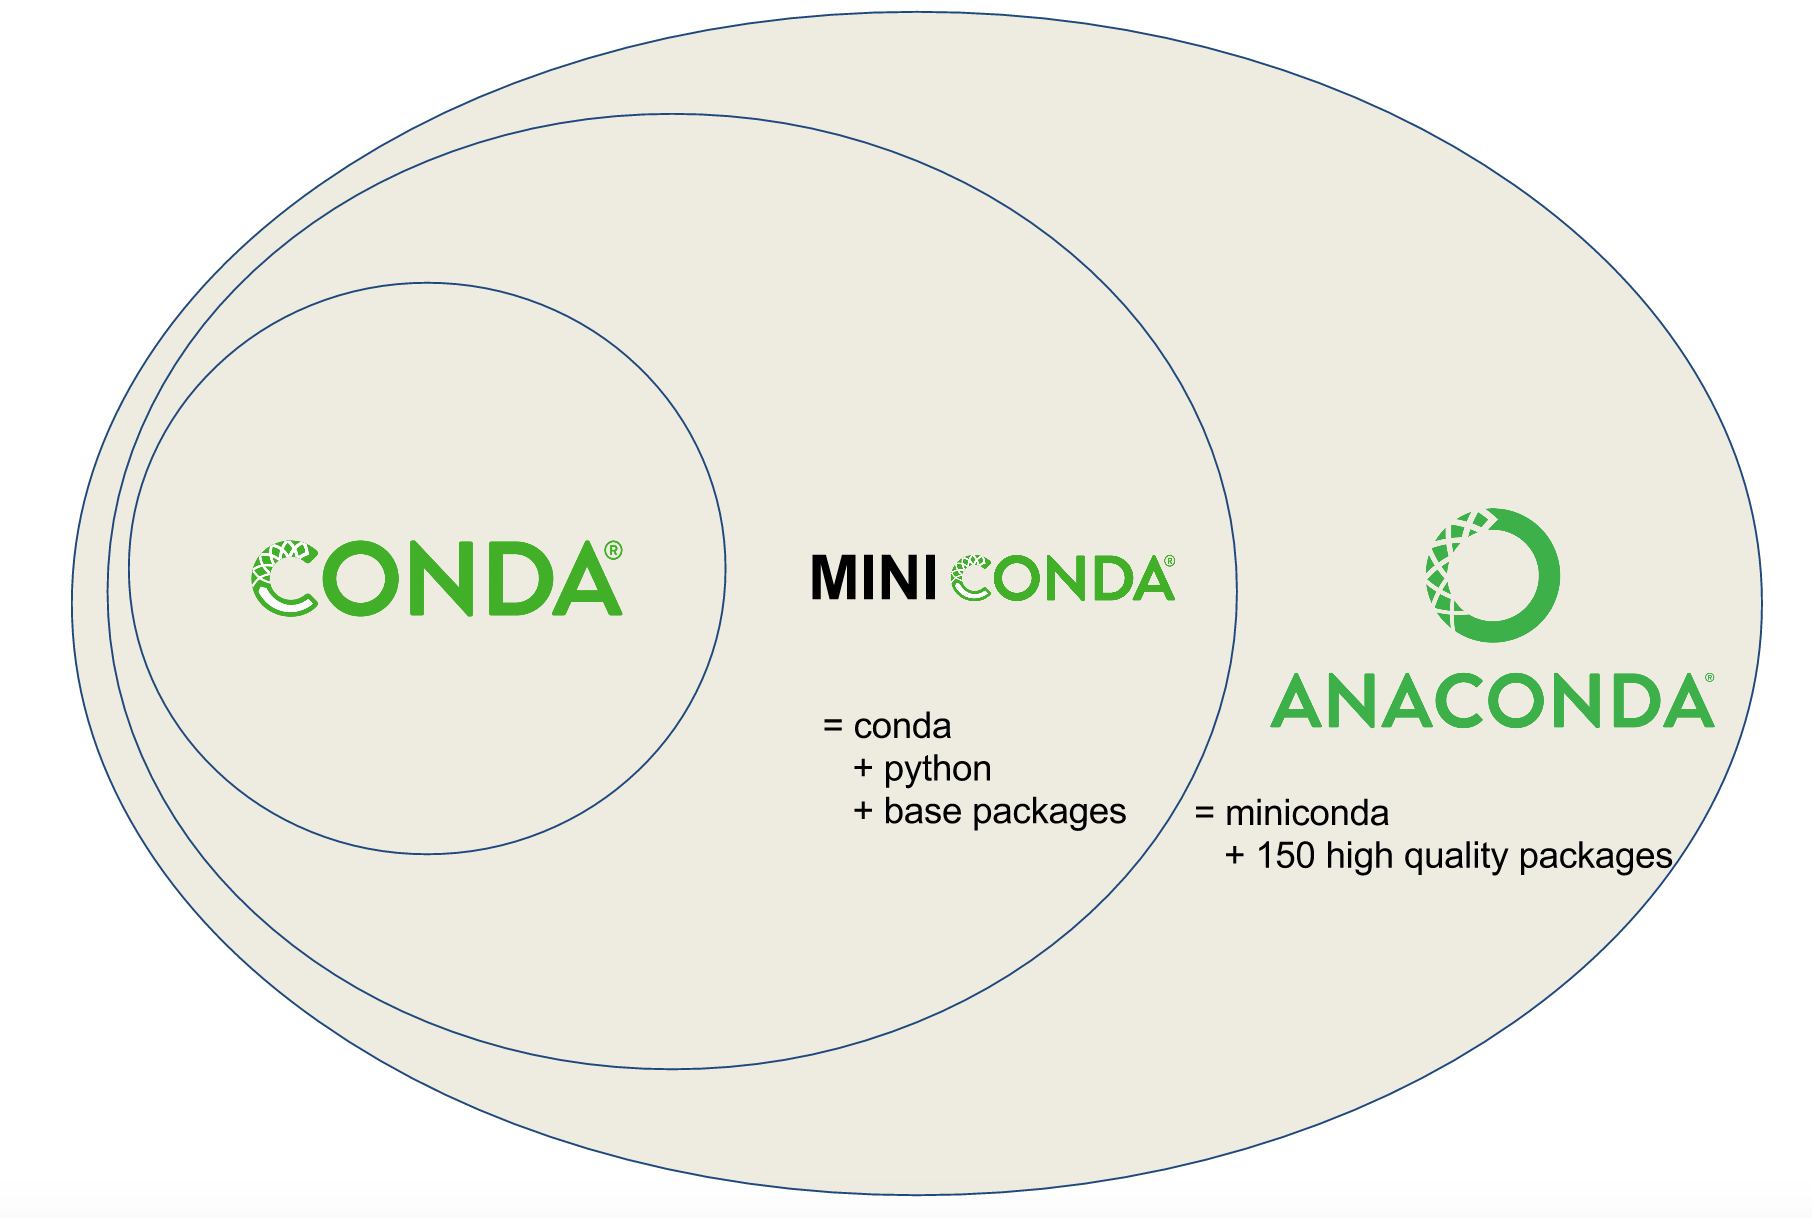
\includegraphics[width=\textwidth]{graphics/conda_mini_ana.png}
    \caption{Relationship between \conda, \texttt{miniconda}, and \texttt{anaconda}.}
    \label{fig:conda_mini_ana}
\end{marginfigure}

\section{Downloading}

\section{Installation}

\subsection{Testing}

\subsection{Updating}

\subsection{Common problems}

\section{Installing libraries}
like \texttt{numpy}, \texttt{matplotlib}, \texttt{pandas}, \texttt{scikit-learn}, and \texttt{networkx}

\section{Maintaining libraries}

\section{Removing libraries}

\section{Environments}